\typeout{NT FILE chapter5.tex}
\chapter{Training the model on more data and model performance evaluation} \label{new_data_train}
\paragraph{}
In section \ref{rs_data_collection} \gls{JP2} data is introduced as a larger dataset sourced to address the issues of bias in data collection. This chapter is dedicated to the evaluation of the impact of using such data on the model fine-tuned on the smaller \gls{GEE} dataset through the experiments in Chapter \ref{experiments_chapter}.

\section{Using transfer learning to train the model on more data}
\paragraph{}
The model was frozen using the best hyperparameters at the end of the Chapter \ref{experiments_chapter} and the model was trained on new data using those weights, this will be compared with the performance of training the model from scratch on new data in section \ref{new_data_train}, the same \gls{ES} strategy will be used for this experiment to prevent overfitting. Using the weights of the previous model trained on the \gls{GEE} data to retrain using new \gls{JP2} data is in essence the same as using transfer learning techniques.

\begin{figure}[hbt!]
    \centering
    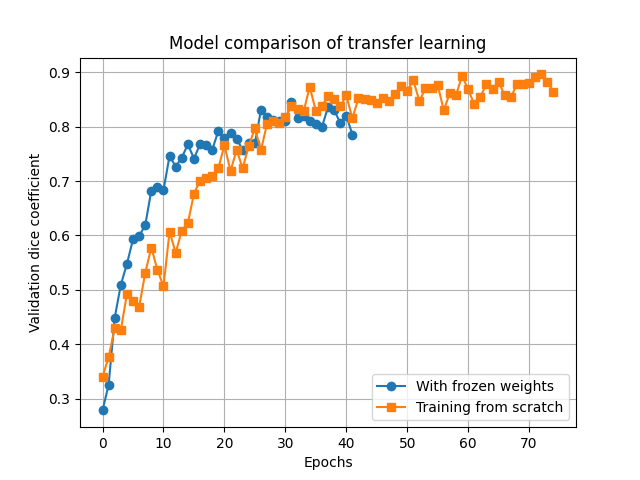
\includegraphics[width=0.75\linewidth]{transfer learning_Validation dice coefficient.png}
    \caption{Retraining with frozen weights Dice Coefficient comparison}
    \label{rt_dice}
\end{figure}

Using the frozen weights did not improve model performance, it had the opposite effect which is expected since the original model has a smaller dataset than the one it was trained on now. It can be seen from Figure \ref{rt_dice} that up to $20$ epochs the transfer learning, by using frozen weights from the model trained on less data, is performing better than the model training from scratch. 

Early stopping is also triggered in the model using frozen weights around $30$ epochs before the model being trained from scratch, which makes sense since when there is less data the model has a greater likelihood of overfitting.

\section{Training the model from scratch on new data} \label{new_data_fs}
\subsection{Comparison with the Google Earth Engine (GEE) dataset model - same parameters}
\paragraph{}
With the same model architecture and hyperparameters as in the previous Chapter, the \gls{DL} model was trained on the \textit{JP2 data} for the same number of epochs to evaluate the effect of using more data on the model performance.

\begin{figure}[hbt!]
    \centering
    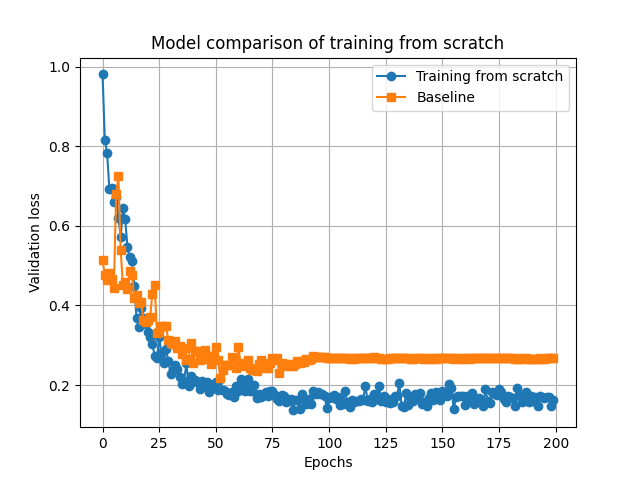
\includegraphics[width=0.75\textwidth]{training from scratch_Validation loss.png}
    \caption{Retraining from scratch Loss comparison}
    \label{fs_loss}
\end{figure}
As can be seen from Figure \ref{fs_loss} the model trained on more data has a lower validation loss consistently after $20$ epochs despite initialising with a higher validation loss, which shows its better performance. 

In terms of evaluation metrics, it can be seen from Table \ref{tab_fs} that the improvement in performance is the most evident in the Test dataset where there is an improvement of $0.08$ in the dice coefficient metric when using \gls{ES} to prevent overfitting.

\begin{table}[ht] 
    \begin{center}
    \begin{tabular}{ccccccc} 
    \toprule
       & \multicolumn{3}{c}{Dice Coefficient}     & \multicolumn{3}{c}{Loss} \\
    Model type & Validation & Training & Test & Validation & Training & Test \\ \midrule
    \rowcolor{lightgray}
    Training from scratch & 0.89 & 0.96 & 0.88 & 0.16 & 0.05 & 0.28  \\ Training from scratch with ES & 0.86 & 0.94 & 0.86 & 0.2 & 0.08 & 0.3  \\ Baseline model & 0.88 & 0.97 & 0.82 & 0.27 & 0.05 & 0.27  \\ Baseline Model with ES & 0.88 & 0.96 & 0.78 & 0.26 & 0.07 & 0.33  \\
    \bottomrule
    \end{tabular}
  \end{center} 
  \caption{Retraining on new data comparison of Dice coefficient and Loss}\label{tab_fs}
\end{table}

\subsection{Hyperparameter tuning from scratch} \label{hp_new_data}
\paragraph{}
What works well for a dataset in terms of hyperparameters may not work well for another, especially when there is a considerable difference in sample size. With this in mind, hyperparameter tuning using random search was performed on the new data with the following parameter variations using the same Early Stopping strategy as before, restoring the weights of the best performing epoch \gls{w.r.t.} Validation Loss:
\begin{itemize}
    \item{Learning Rate: 0.0001 and 0.001}
    \item{Optimiser: RMSprop, Adam and Nadam}
    \item{Loss Function: CE Dice Loss}
    \item{Batch Size: 1 and 10}
    \item{Activation Function: ELU}
    \item{Initialisation Method: He Normal}
\end{itemize}

Results were logged using Tensorboard, the best validation dice coefficient combinations of hyperparameters are shown in Figure \ref{hp}, the best hyperparameters for the \gls{JP2} data were batch size of $10$, \gls{RMSProp} optimiser and learning rate of $0.001$.

\begin{figure}[hbt!]
    \centering
    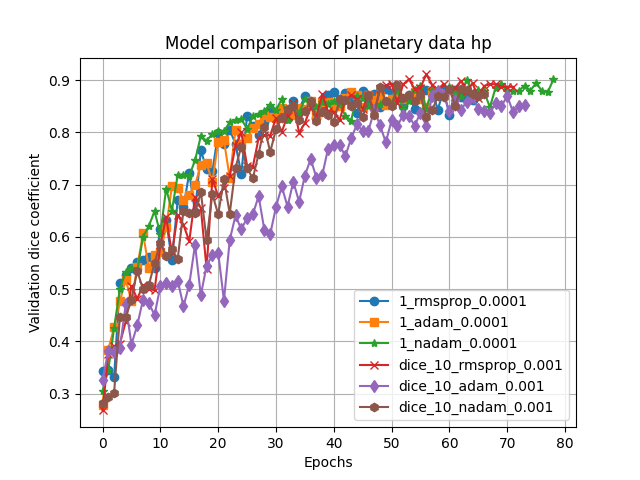
\includegraphics[width=0.75\linewidth]{planetary data hp_Validation dice coefficient.png}
    \caption{Subset of hyperparameter experiments with new data Validation dice coefficient}
    \label{hp}
\end{figure}
As it can be seen from Table \ref{tab_hp} the difference in performance with regards to the Validation Dice Coefficient is marginal between the different hyperparameter combinations, showing that the previous experiments in Chapter \ref{experiments_chapter} provided good insights that generally apply to a different bigger dataset.

\begin{table}[ht!] 
    \begin{center}
    \begin{tabular}{ccccccc} 
    \toprule
       & \multicolumn{3}{c}{Dice Coefficient}     & \multicolumn{3}{c}{Loss} \\
    Hyperparameter combination & Validation & Training & Test & Validation & Training & Test \\ \midrule
%\rowcolor{lightgray}
    1 rmsprop 0.0001 & 0.86 & 0.94 & 0.93 & 0.2 & 0.07 & 0.15  \\ 1 adam 0.0001 & 0.87 & 0.93 & 0.91 & 0.19 & 0.09 & 0.14  \\ 1 nadam 0.0001 & 0.86 & 0.93 & 0.76 & 0.2 & 0.09 & 0.22  \\ \rowcolor{lightgray}10 rmsprop 0.001 & 0.91 & 0.96 & 0.95 & 0.13 & 0.05 & 0.11  \\ 10 adam 0.001 & 0.6 & 0.68 & 0.64 & 0.55 & 0.44 & 0.36  \\ 10 nadam 0.001 & 0.59 & 0.72 & 0.84 & 0.56 & 0.38 & 0.33  \\
\bottomrule
    \end{tabular}
  \end{center} 
  \caption{Hyperparameter combinations comparison of Dice Coefficient and Loss}\label{tab_hp}
\end{table}

\section{Final Model}
\paragraph{}
The best model found was that from the hyperparameter tuning performed on the new \textit{JP2} data in Section \ref{hp_new_data}, the performance of this model was summarised in Table \ref{tab_hp}, which shows a Dice Score on the test dataset of $95\%$. More in-depth analysis per epoch will now be performed in this section.

As it can be seen from Figure \ref{best_loss}, there is no evidence of overfitting before the Early Stopping strategy kicks off at the 88th epoch. It can also be seen from Figure \ref{best_dice}, that the Training and Validation curve follow a similar shape with less fluctuation towards the final epochs, as would be expected from a well-performing model.

\begin{figure}[hbt!]
    % \centering
    \begin{minipage}[c]{0.5\linewidth}
    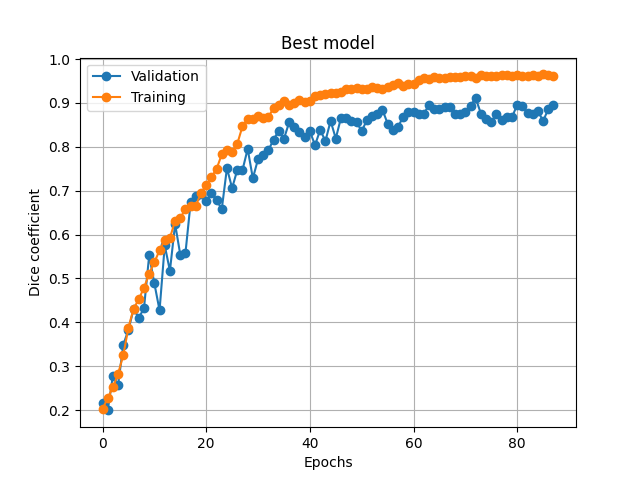
\includegraphics[width=\linewidth]{Best model_Dice coefficient.png}
    \caption{Dice Score comparison}
    \label{best_dice}
    \end{minipage}
        \hfill
        \begin{minipage}[c]{0.5\linewidth}
        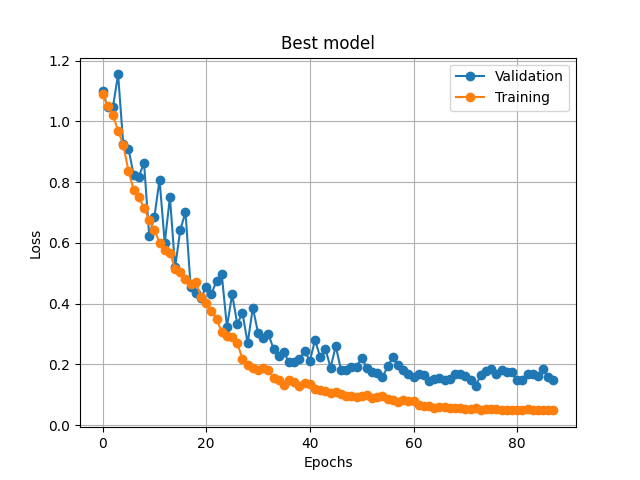
\includegraphics[width=\linewidth]{Best model_Loss.png}
        \caption{Loss
        comparison}
        \label{best_loss}
    \end{minipage}
\end{figure}

\section{Test Evaluation}
\paragraph{}
During the Training/ Validation/ Test split process $39$ images were assigned to the test set, that is completely unseen data by the model. Using the best model's frozen weights (the best weights are restored as part of the \gls{ES} strategy) and architecture, inference is performed of the test dataset to assess model performance by comparing the predictions against the ground truth mask.
The overall performance of the model at image level is summarised in Table \ref{sum_test}, where three categories are defined according to model performance, the individual performance evaluation scores of each test image are then compared in Figure \ref{scatter_test_scores} according to those categories.
    \begin{table}[!h] 
        \begin{center}
        \begin{tabular}{ccc} 
        \toprule
        \textbf{Category} & \textbf{Dice Score range} & \textbf{Number of images} \\ \midrule
        High & Greater than or equal to 0.7 & 29  \\
        Medium & Between 0.7 and 0.4 & 5  \\
        Low & Smaller or equal to 0.4 & 5  \\
    \bottomrule
        \end{tabular}
      \end{center} 
      \caption{Dice score test image summary}\label{sum_test}
    \end{table}
    \begin{figure}[hbt!]
        \centering
        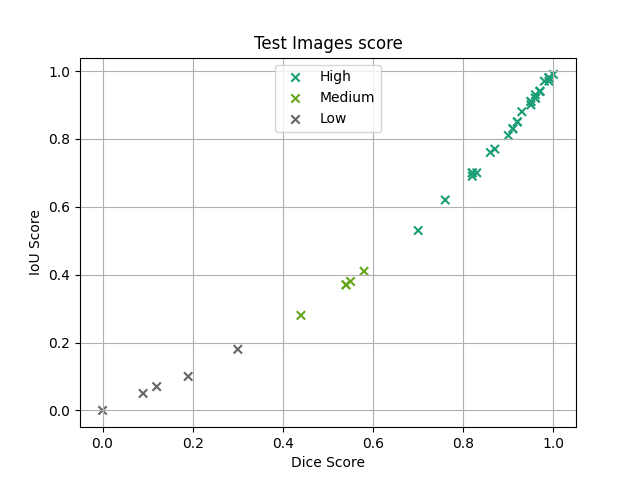
\includegraphics[width=0.75 \textwidth]{test images scores.png}
        \caption{Dice Score vs. IoU Score Test images scatter plot}
        \label{scatter_test_scores}
    \end{figure}

A short image-by-image analysis will be performed for two images of each category, where purple colour represents background (non-\gls{RTS}) pixels and yellow represents foreground (\gls{RTS}) pixels. The pixels have varying opacity according to prediction confidence where the lighter the shade the lower the confidence and there is also a red contour which represents the ground truth mask outline.

As can be seen from Figure \ref{high_score_pic} the algorithm can deal with both simpler thaw slump shapes (on the left) and more complex shapes (on the right), although the latter shows lower confidence in the pixel prediction confidence, as can be seen by lower intensity pixel shading and is also reflected in a lower dice score.
    \begin{figure}[htp]
        % \centering
        \begin{minipage}[l][][c]{0.45\linewidth}
        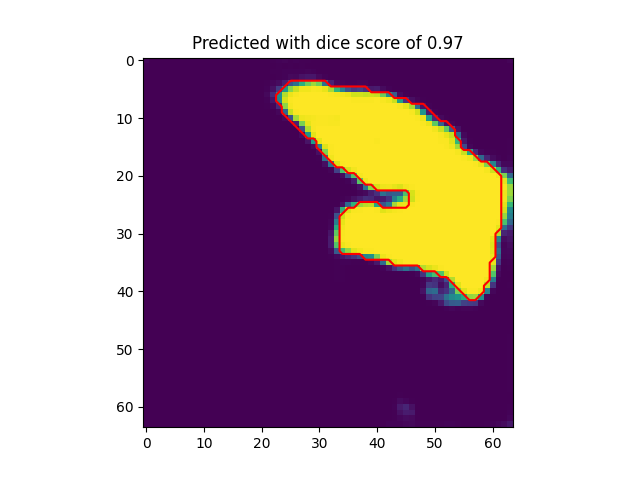
\includegraphics[width=\linewidth]{1_0.97.png}
        \end{minipage}
        \hfill
        \begin{minipage}[r][][c]{0.45\linewidth}
        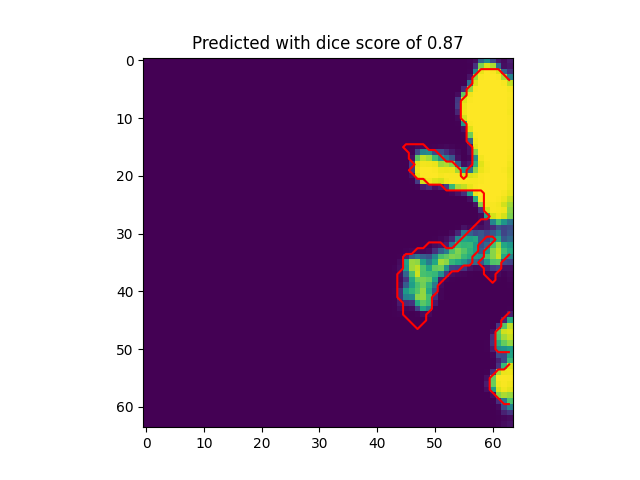
\includegraphics[width=\linewidth]{25_0.87.png}
        \end{minipage}
        \caption{Test set predicted vs. ground truth high score examples}\label{high_score_pic}
    \end{figure}

The model struggles with elongated thaw slumps as seen in Figure \ref{medium_score_pic} on the left and in some instances correctly predicts the thaw slump \gls{ROI} but also predicts False Positive \gls{RTS} which then has an impact on the dice score (right side). This presence of False Positives could be an indication of an actual \gls{RTS}, which has not been labeled yet. Due to the lack of expert knowledge, these False Positives have not been validated but could point researchers in the right direction when looking for new \gls{RTS}.
    \begin{figure}[htp]
        % \centering
        \begin{minipage}[c]{0.45\linewidth}
        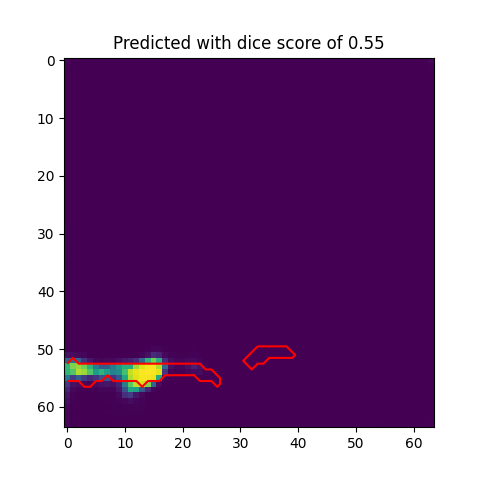
\includegraphics[width=\linewidth]{11_0.55.png}
        \end{minipage}
            \hfill
            \begin{minipage}[c]{0.45\linewidth}
            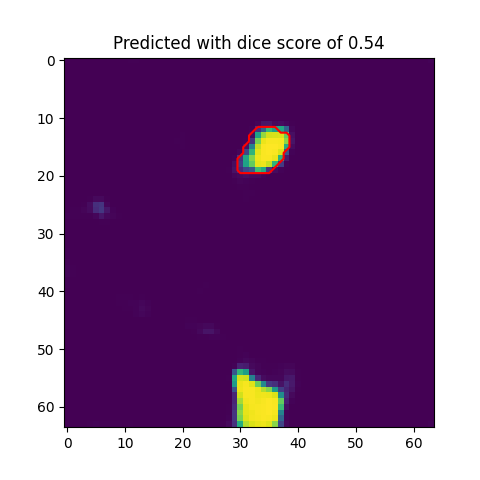
\includegraphics[width=\linewidth]{10_0.54.png}
        \end{minipage}
        \caption{Test set predicted vs. ground truth medium score examples} \label{medium_score_pic}
    \end{figure}

 The really low performing test images can be seen in Figure \ref{low_score_pic}, the model seems to not be very good at predicting very small \gls{RTS}, this could be due to the fact that each pixel represents a \SI{10}{\metre\squared} area and some \gls{RTS} may be smaller than that, or that the image reprojection has a slight misalignment, as can be seen from the image on the left which predicts a False Positive \gls{RTS} to the left of the ground truth red contour.
    \begin{figure}[htp]
        \begin{minipage}[c]{0.45\linewidth}
        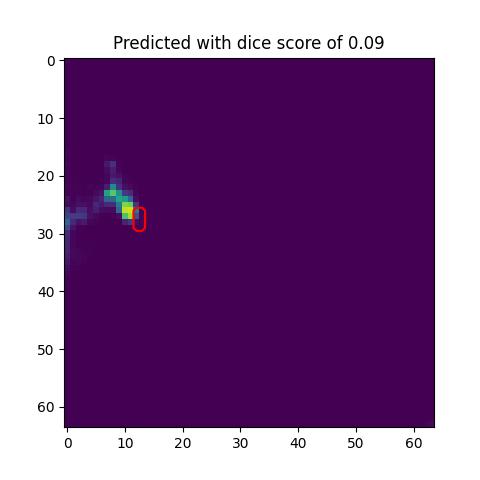
\includegraphics[width=\linewidth]{19_0.09.png}
        \end{minipage}
            \hfill
            \begin{minipage}[c]{0.45\linewidth}
            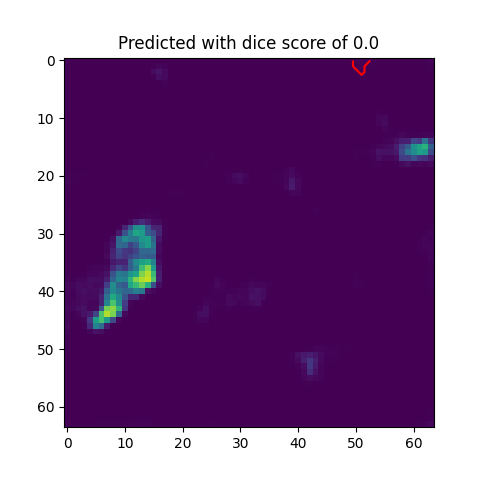
\includegraphics[width=\linewidth]{31_0.0.png}
        \end{minipage}
        \caption{Test set predicted vs. ground truth low score examples} \label{low_score_pic}
    \end{figure}

Another level of analysis involves looking at the input images ($X$) next to the ground truth and predictions ($y$ and predicted $y$) to check if there is any visible evidence to analyse, an example of this can be seen in Figure \ref{medium_score_input_pic}. By analysing the input image (on the left), it can be seen that the image is corrupted at the top, this could be perhaps due to an error in the multispectral instrument during the collection. When it comes to the \gls{RTS} \gls{ROI}, the lighter shading in the input image corresponds to the predicted area on the right side, indicating that perhaps the reprojection of the labelled data (red contour) to the input image's \gls{CRS} is incorrect and the algorithm is indeed more accurate than the dice score of $58\%$ seems to suggest. This could be likely since the ground truth was sourced from Planet imagery whilst the input image was sourced from Satellite-2.
\begin{figure}[htp]
    \centering
    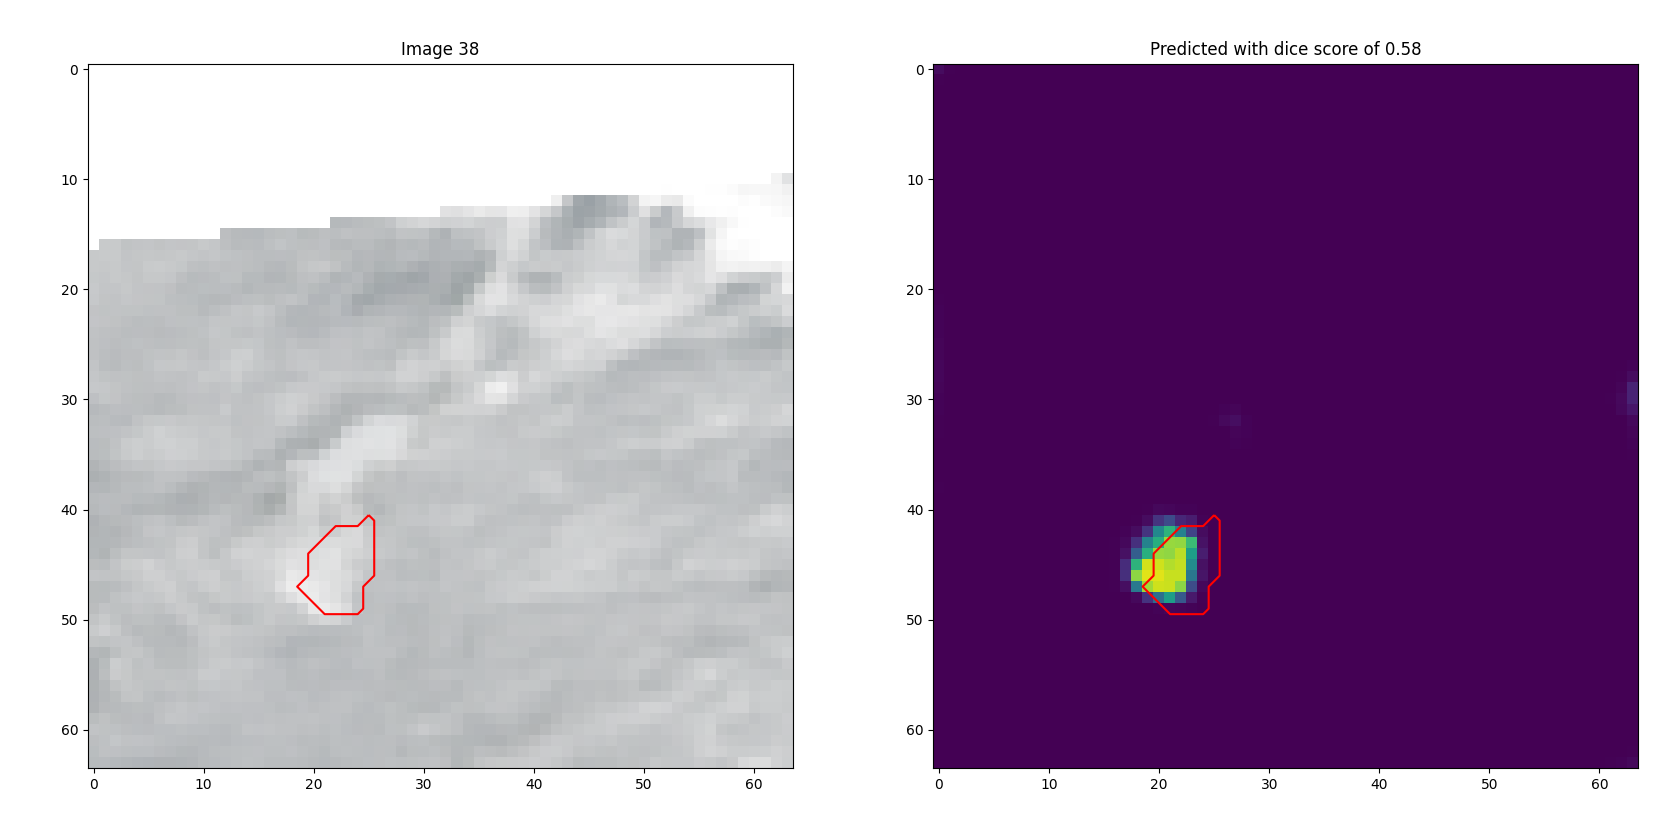
\includegraphics[width=0.75\textwidth]{38_0.58_input.png}
    \caption{Test set predicted vs. ground medium score example}
    \label{medium_score_input_pic}
\end{figure}

Given more time, all the above assumptions would be investigated further.
